\section{Experimental Results}
\label{sec:results}

All experiments use the reference dataset described in
Section~\ref{sec:method:ref}: $D = 2{,}000$ traces, $T = 29{,}000$ samples.

\subsection{CPA Key Recovery}

Table~\ref{tab:cpa} summarises CPA results for all 16 key bytes.
The attack was run with leakage constant $c$ swept from 0 to 255.
Key recovery verified (via backward key schedule against the known key) at
$c = 2$.

\begin{table}[H]
\centering
\caption{CPA last-round key recovery. Rank = rank of correct round-10 byte
         among 256 hypotheses. All 16 bytes at rank 1; $c=2$ used.}
\label{tab:cpa}
\begin{tabular}{@{}ccccc@{}}
\toprule
Byte & Correct $k_{10,b}$ & CPA guess & Rank & Const needed \\
\midrule
 0  & \texttt{D0} & \texttt{D0} & 1 & 0 \\
 1  & \texttt{14} & \texttt{14} & 1 & 0 \\
 2  & \texttt{F9} & \texttt{F9} & 1 & 0 \\
 3  & \texttt{A8} & \texttt{A8} & 1 & 0 \\
 4  & \texttt{C9} & \texttt{C9} & 1 & 0 \\
 5  & \texttt{EE} & \texttt{EE} & 1 & 0 \\
 6  & \texttt{25} & \texttt{25} & 1 & 0 \\
 7  & \texttt{89} & \texttt{89} & 1 & 0 \\
 8  & \texttt{E1} & \texttt{E1} & 1 & 0 \\
 9  & \texttt{3F} & \texttt{3F} & 1 & 0 \\
10  & \texttt{0C} & \texttt{0C} & 1 & 0 \\
11  & \texttt{C8} & \texttt{D1} & \textbf{2} & \textbf{2} \\
12  & \texttt{B6} & \texttt{B6} & 1 & 0 \\
13  & \texttt{63} & \texttt{63} & 1 & 0 \\
14  & \texttt{0C} & \texttt{0C} & 1 & 0 \\
15  & \texttt{A6} & \texttt{A6} & 1 & 0 \\
\bottomrule
\end{tabular}
\end{table}

Fifteen bytes are recovered at rank 1 with the pure HW model ($c=0$).
Byte 11 requires $c=2$, indicating the leakage for that byte follows an HD
model (transitions from value 2).
This is consistent with the reference notebook results on the same dataset.
With $c=2$ the full 128-bit original key is recovered:
\texttt{2B 7E 15 16 28 AE D2 A6 AB F7 15 88 09 CF 4F 3C}.

Figure~\ref{fig:cpa} shows the three-panel CPA diagnostic for byte 0
(correct hypothesis $j = \texttt{0xD0}$).

\begin{figure}[H]
  \centering
  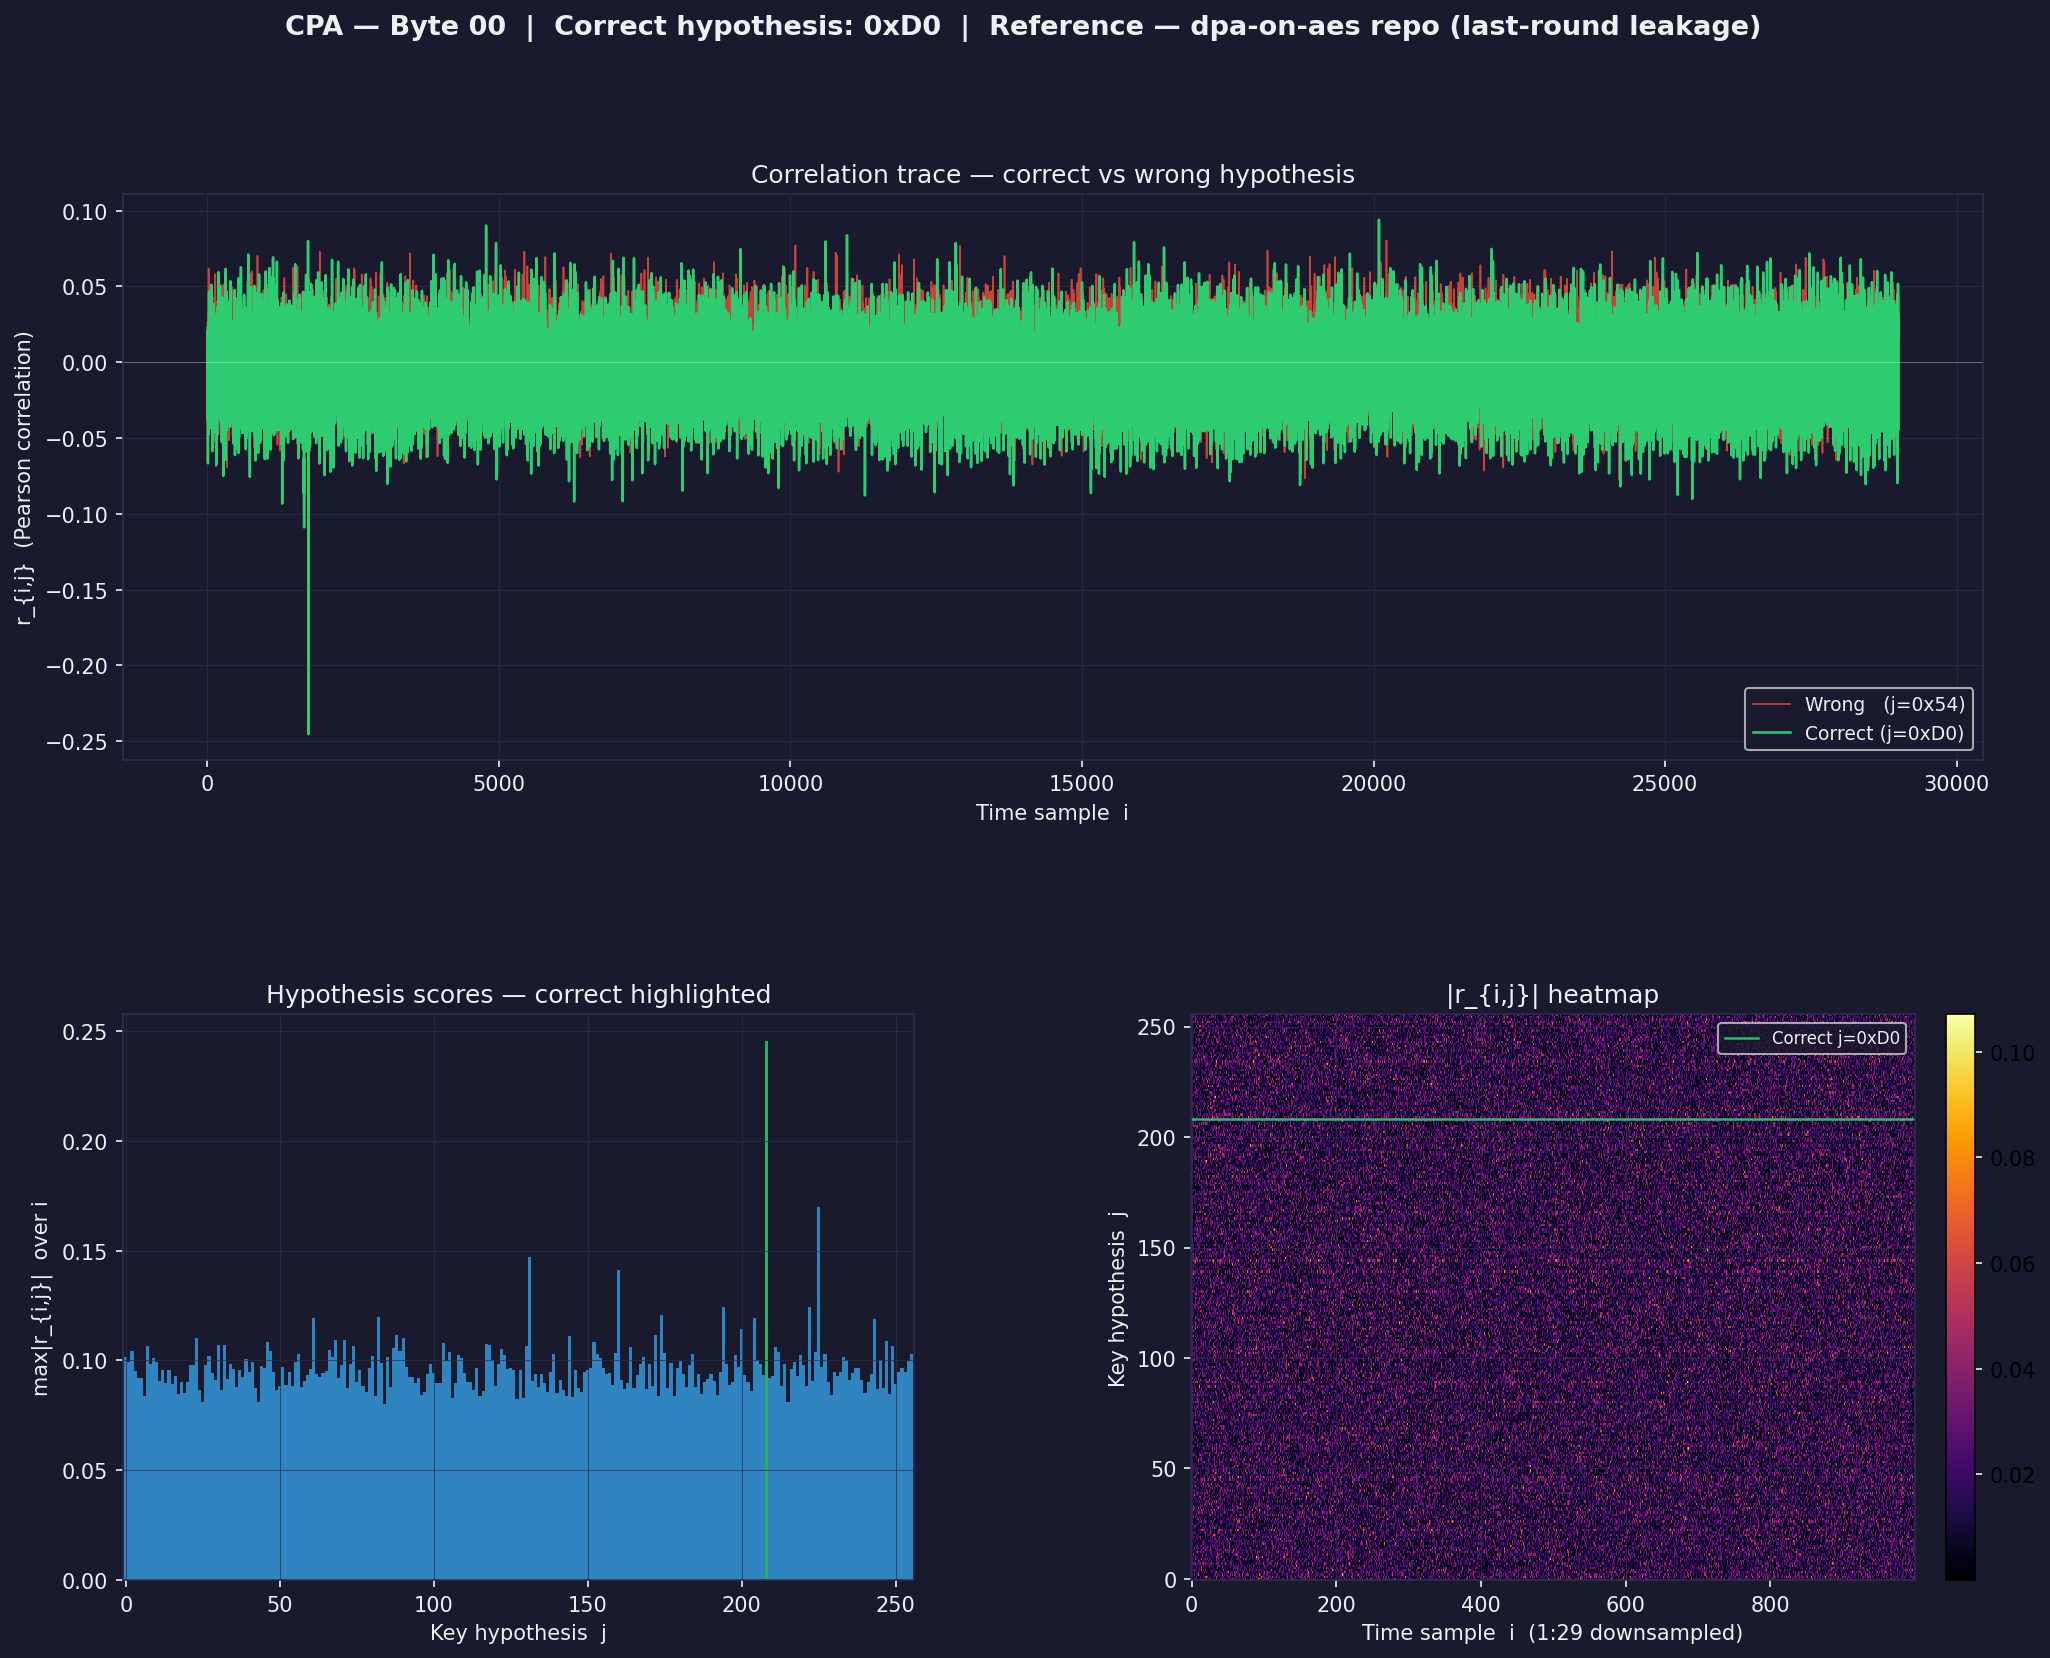
\includegraphics[width=\linewidth]{figures/cpa_byte00.png}
  \caption{CPA diagnostic for key byte 0, $c=2$.
           \textbf{Top}: correlation $r_{i,j}$ over all 29{,}000 time samples
           for the correct hypothesis (green, $j=\texttt{0xD0}$) vs. a wrong
           one (red, $j=\texttt{0x54}$, lowest-scoring).
           The correct guess shows a pronounced negative spike near sample
           1{,}000, corresponding to the last-round SubBytes operation.
           \textbf{Bottom-left}: max $|r_{i,j}|$ across all time samples for
           each of the 256 hypotheses; correct hypothesis (green bar)
           stands clearly above the noise floor.
           \textbf{Bottom-right}: $|r_{i,j}|$ heatmap; the correct
           hypothesis row is the brightest band.}
  \label{fig:cpa}
\end{figure}

\subsection{DPA Key Recovery}

DPA was run with bit position $\ell$ swept from 0 to 7.
Full key recovery was achieved at $\ell = 1$.

\begin{itemize}
  \item \textbf{Bit 0}: 14/16 bytes correct; bytes 3 and 15 wrong.
        Backward key schedule fails verification.
  \item \textbf{Bit 1}: 16/16 bytes correct.
        Recovered round-10 key:
        \texttt{D0 14 F9 A8 C9 EE 25 89 E1 3F 0C C8 B6 63 0C A6}.
        Original key: \texttt{2B 7E 15 16 28 AE D2 A6 AB F7 15 88 09 CF 4F 3C}.
\end{itemize}

Figure~\ref{fig:dpa} shows the DPA diagnostic for byte 0, bit $\ell = 1$.

\begin{figure}[H]
  \centering
  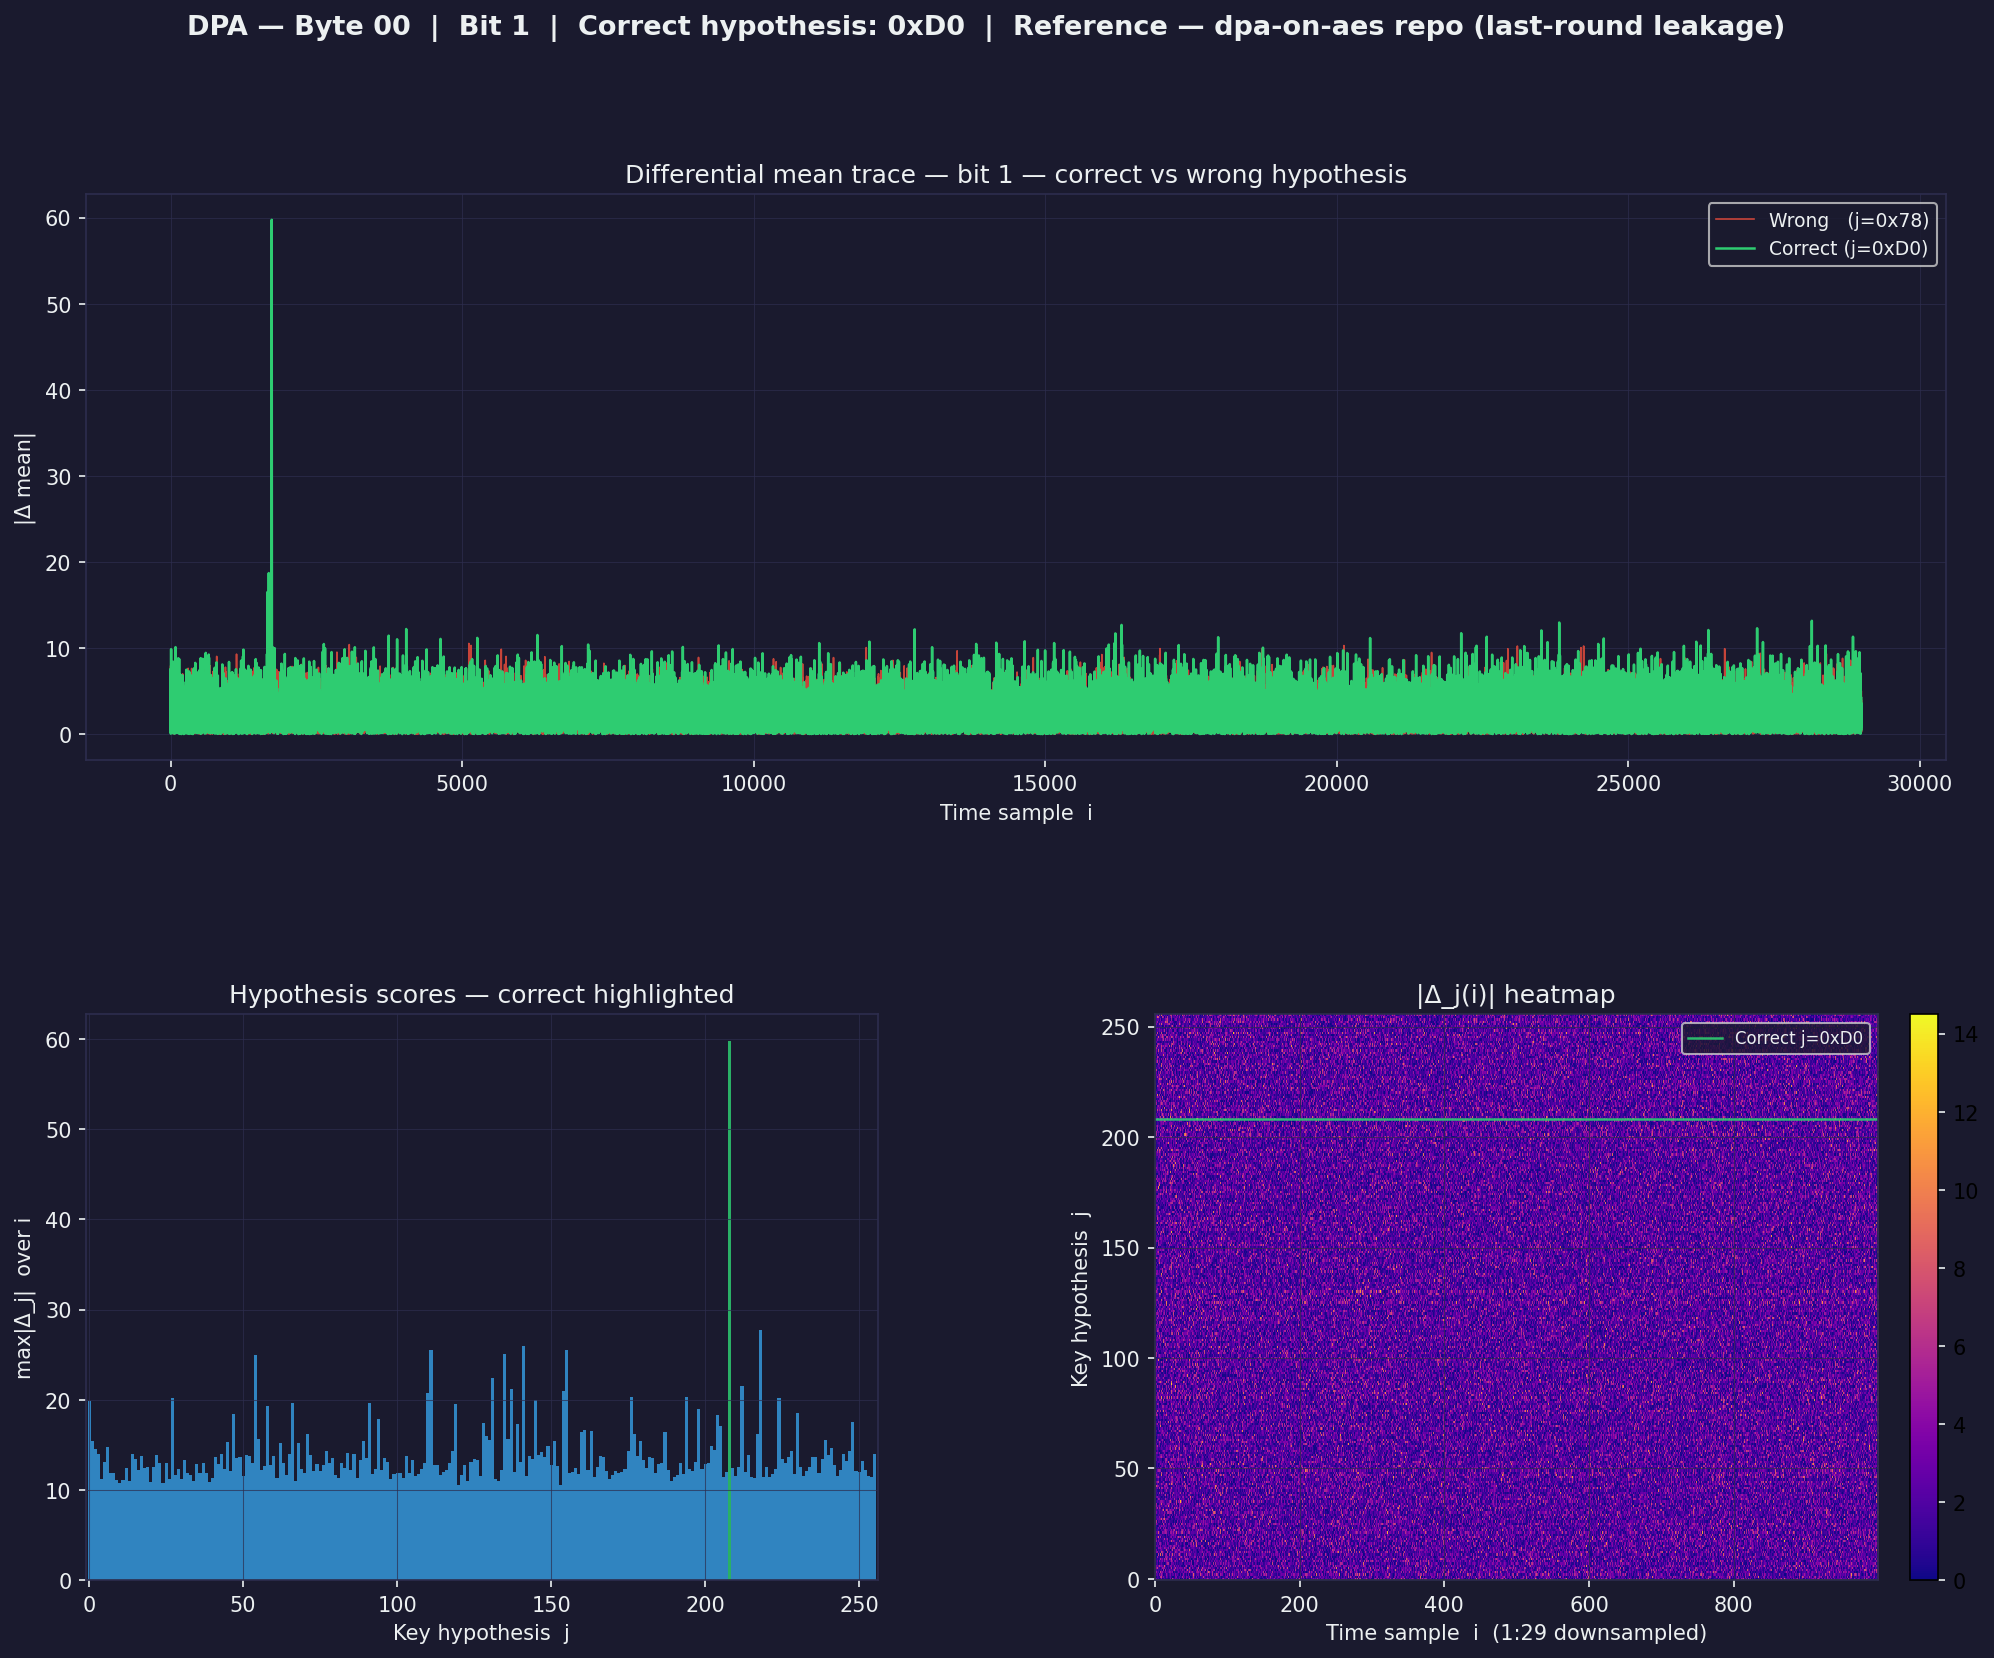
\includegraphics[width=\linewidth]{figures/dpa_byte00_bit1.png}
  \caption{DPA diagnostic for key byte 0, bit $\ell = 1$.
           \textbf{Top}: differential mean $\Delta_j(i)$ over 29{,}000 time
           samples; the correct hypothesis (green, $j=\texttt{0xD0}$) shows a
           sharp peak near the last-round SubBytes window while the wrong
           hypothesis (red) is flat.
           \textbf{Bottom-left}: distinguisher scores for all 256 hypotheses.
           \textbf{Bottom-right}: full $\Delta_j(i)$ heatmap.}
  \label{fig:dpa}
\end{figure}

\subsection{Guessing Entropy}
\label{sec:results:ge}

% ── TODO ──────────────────────────────────────────────────────────────────────
% GE curves require running attacks/guessing_entropy.py on a trace set.
% Once real hardware traces (set_001_pico_real) are collected, replace this
% placeholder with the actual GE vs N_traces plots.
% ─────────────────────────────────────────────────────────────────────────────

\textbf{Note:} Guessing Entropy curves comparing DPA and CPA as a function of
trace count $N$ are pending real hardware trace acquisition
(dataset \texttt{set\_001\_pico\_real}).
The script \texttt{attacks/guessing\_entropy.py} automates GE estimation via
random subsampling trials and will populate this section once traces are
collected.
A placeholder figure location is reserved here for the final submission.

\begin{figure}[H]
  \centering
  \fbox{\parbox{0.9\linewidth}{\centering\vspace{2cm}
    \textit{[PLACEHOLDER]} \\
    GE vs.\ $N_\text{traces}$ for CPA and DPA on \texttt{set\_001\_pico\_real}. \\
    Generated by \texttt{attacks/guessing\_entropy.py --data data/set\_001\_pico\_real}
    \vspace{2cm}}}
  \caption{Guessing Entropy comparison: DPA vs.\ CPA on real Pico hardware
           traces. Target: key byte 0. Horizontal dashed line at GE\,=\,1
           marks full convergence.}
  \label{fig:ge}
\end{figure}
